\subsection{Ablation Study, Parameter Sensitivity, and Efficiency Analysis}
\label{sec:exp_ablation}

\begin{table}[!t]
\centering
\begin{threeparttable}
\caption{Component Ablation Study of SP-PD}
\label{tab:ablation}
\scriptsize
\setlength{\tabcolsep}{3.8pt}
\renewcommand{\arraystretch}{1.07}
\begin{tabular}{@{}lrrrrr@{}}
\toprule
\multicolumn{6}{@{}l}{\textbf{Clinical Datasets ($n = 30$, $K = 4$, $B = 128$)}} \\
\addlinespace[2pt]
Variant & Aln. & Mis. & Mean\tnote{a} & LR\tnote{a} & RF\tnote{a} \\
\midrule
w/o Prior                      & 65.87 & 65.87 & 65.87\rlap{\textsuperscript{*}} & 65.55\rlap{\textsuperscript{*}} & 63.20\rlap{\textsuperscript{*}} \\
w/o Search                     & \textbf{66.97} & 59.29 & 63.13\rlap{\textsuperscript{*}} & 62.78\rlap{\textsuperscript{*}} & 61.26\rlap{\textsuperscript{*}} \\
w/o Prior Reg. ($\lambda{=}0$) & 65.91 & \textbf{65.96} & 65.94\rlap{\textsuperscript{*}} & 65.55\rlap{\textsuperscript{*}} & 63.26\rlap{\textsuperscript{*}} \\
w/o Rep. Pairing ($R{=}1$)     & 66.62 & 65.60 & 66.11 & 65.65 & 63.60 \\
\midrule
SP-PD                          & 66.65 & 65.85 & \textbf{66.25} & \textbf{65.75} & \textbf{63.67} \\
\midrule
\multicolumn{6}{@{}l}{\textbf{High-Dimensional Benchmarks ($K = 8$, $B = 1{,}000$)}} \\
\addlinespace[2pt]
Variant & $B{=}128$ & $B{=}1{,}000$ & BA & F1 & CPU (s) \\
\midrule
w/o Error-Guided Search   & 76.08 & 75.62 & 71.39 & 71.67 & \textbf{3.16} \\
w/o Tree-Union Proposal   & 76.21 & 76.11 & 71.56 & 72.02 & 4.34 \\
\midrule
SP-PD                     & \textbf{76.61} & \textbf{76.52} & \textbf{71.98} & \textbf{72.46} & 4.43 \\
\bottomrule
\end{tabular}
\begin{tablenotes}[flushleft]
\scriptsize
\item[a] Aln., Mis., and Mean report NC BA (\%); LR and RF report unweighted aligned/misaligned mean BA (\%) at $n = 30$. High-dimensional columns report macro-precision (\%), BA (\%), macro-F1 (\%), and mean CPU time across 23 groups.
\item[*] SP-PD significantly outperforms the ablated variant (Wilcoxon, $\alpha = 0.05$).
\end{tablenotes}
\end{threeparttable}
\end{table}

\begin{table}[!t]
\centering
\begin{threeparttable}
\caption{LLM Query Cost and Stochastic Prompt Stability}
\label{tab:efficiency_stability}
\scriptsize
\setlength{\tabcolsep}{2.8pt}
\renewcommand{\arraystretch}{1.07}
\begin{tabular}{@{}lrrrr@{}}
\toprule
\multicolumn{5}{@{}l}{\textbf{Offline LLM Query and Token Cost}} \\
\addlinespace[2pt]
Algorithm & Calls\tnote{a} & Out. Tok. & Peak Tok. & API (s) \\
\midrule
LLM-Select (Score) / LSP & 3.2 / 26 & 1,054.3 & 10,387 & 27.6 \\
LLM-Lasso                & 3.2 / 26 &   777.8 &  7,817 & 31.3 \\
\midrule
SP-PD                    & \textbf{1.0 / 1} & \textbf{59.3} & \textbf{68} & \textbf{13.8} \\
\midrule
\multicolumn{5}{@{}l}{\textbf{Five-Run Prompt Stability (Mean $\pm$ SD \%)}} \\
\addlinespace[2pt]
 & \multicolumn{2}{c}{$n = 3$} & \multicolumn{2}{c}{$n = 30$} \\
\cmidrule(lr){2-3} \cmidrule(l){4-5}
Algorithm & Aln. & Mis. & Aln. & Mis. \\
\midrule
LLM-Select (Rank) & \textbf{56.14}$\pm$0.45 & 51.38$\pm$0.12 & \textbf{63.53}$\pm$0.62 & 54.29$\pm$0.22 \\
SP-PD             & 55.09$\pm$\textbf{0.16} & \textbf{54.64}$\pm$\textbf{0.10} & 61.77$\pm$\textbf{0.25} & \textbf{60.72}$\pm$\textbf{0.05} \\
\bottomrule
\end{tabular}
\begin{tablenotes}[flushleft]
\scriptsize
\item[a] Mean / maximum batched offline calls across the 12 clinical datasets; native per-feature prompting for LLM-Select (Score) requires 78.9 mean and 753 maximum calls. Stability is evaluated over five independent prompts on six clinical datasets.
\end{tablenotes}
\end{threeparttable}
\end{table}


\begin{figure*}[!t]
\centering
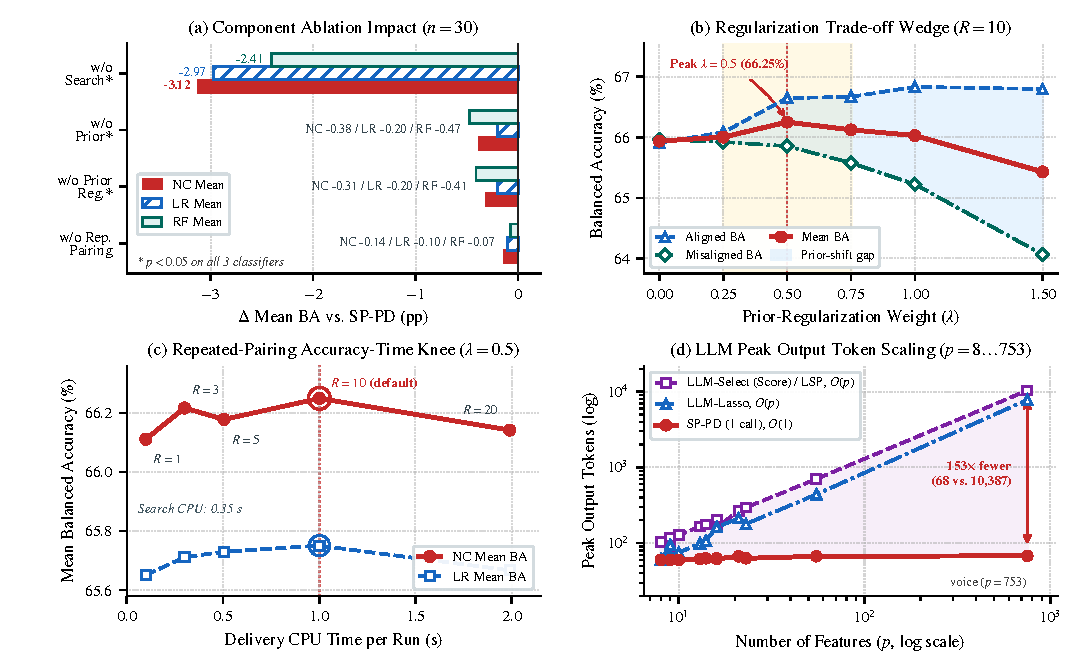
\includegraphics[width=\textwidth]{figures/fig3_ablation_sensitivity_cost.pdf}
\caption{Component ablation impact, hyperparameter sensitivity, delivery runtime trade-off, and $O(1)$ versus $O(p)$ LLM token scaling.}
\label{fig:ablation_sens_cost}
\end{figure*}

As shown in Table~\ref{tab:ablation} and Fig.~\ref{fig:ablation_sens_cost}(a), removing any single module of SP-PD degrades generalization across all three classifiers on the 12 clinical datasets. Dropping the offline semantic prior reduces SP-PD to a purely data-driven selector and significantly lowers NC, LR, and RF means. Removing evolutionary search collapses misaligned accuracy by 6.56 percentage points, yielding significant drops on every classifier. Disabling prior regularization at $\lambda = 0$ preserves misaligned recovery but forfeits 0.74 percentage points under aligned priors, significantly lowering all three means. Restricting delivery to one pairing at $R = 1$ raises validation variance and reduces misaligned recovery by 0.25 percentage points. On the 23 high-dimensional benchmark groups, removing error-guided search drops macro-precision by 0.90 percentage points and macro-F1 by 0.79 percentage points, while removing tree-union proposals degrades all terminal metrics at $B = 1{,}000$.

Fig.~\ref{fig:ablation_sens_cost}(b) shows how $\lambda$ governs the balance between prior exploitation and correction. As $\lambda$ increases from 0 to 1.50, aligned BA rises monotonically while the shaded prior-shift gap widens; overall mean BA stays stable across $[0.25, 1.00]$ and peaks at $\lambda = 0.5$ with 66.25\%. Excessive regularization at $\lambda = 1.50$ impedes correction and drags misaligned BA down to 64.06\%. In Fig.~\ref{fig:ablation_sens_cost}(c), both NC and LR mean BA peak at $R = 10$, where delivery adds 1.00~s on top of 0.35~s search time per clinical run. Increasing $R$ to 20 doubles delivery time without further gain. On the high-dimensional benchmarks in Table~\ref{tab:ablation}, SP-PD averages 4.43~s of CPU time per run at $B = 1{,}000$, adding 1.27~s over random search while raising macro-precision by 0.90 percentage points.

Because SP-PD requests only one offline feature ranking per dataset, Table~\ref{tab:efficiency_stability} and Fig.~\ref{fig:ablation_sens_cost}(d) confirm strictly $O(1)$ query scaling. Across all 12 clinical datasets, SP-PD uses one API call and 59.3 output tokens on average, peaking at 68 tokens on voice at $p = 753$. By contrast, LLM-Lasso and LLM-Select (Score) output per-feature weights or scores that scale as $O(p)$, peaking at 7,817 and 10,387 tokens on voice, up to 153 times higher than SP-PD, while native LLM-Select (Score) needs 753 calls. On six clinical datasets across five independent LLM runs at $T = 0$ and $T = 0.3$, SP-PD cuts across-prompt standard deviation by 60\% under aligned priors and 77\% under misaligned priors at $n = 30$. Evolutionary search and repeated-pairing delivery thus dampen LLM sampling variance.
